\documentclass[]{book}
\usepackage{lmodern}
\usepackage{amssymb,amsmath}
\usepackage{ifxetex,ifluatex}
\usepackage{fixltx2e} % provides \textsubscript
\ifnum 0\ifxetex 1\fi\ifluatex 1\fi=0 % if pdftex
  \usepackage[T1]{fontenc}
  \usepackage[utf8]{inputenc}
\else % if luatex or xelatex
  \ifxetex
    \usepackage{mathspec}
  \else
    \usepackage{fontspec}
  \fi
  \defaultfontfeatures{Ligatures=TeX,Scale=MatchLowercase}
\fi
% use upquote if available, for straight quotes in verbatim environments
\IfFileExists{upquote.sty}{\usepackage{upquote}}{}
% use microtype if available
\IfFileExists{microtype.sty}{%
\usepackage{microtype}
\UseMicrotypeSet[protrusion]{basicmath} % disable protrusion for tt fonts
}{}
\usepackage[margin=1in]{geometry}
\usepackage{hyperref}
\hypersetup{unicode=true,
            pdftitle={biggr},
            pdfauthor={Freddy Drennan},
            pdfborder={0 0 0},
            breaklinks=true}
\urlstyle{same}  % don't use monospace font for urls
\usepackage{natbib}
\bibliographystyle{apalike}
\usepackage{color}
\usepackage{fancyvrb}
\newcommand{\VerbBar}{|}
\newcommand{\VERB}{\Verb[commandchars=\\\{\}]}
\DefineVerbatimEnvironment{Highlighting}{Verbatim}{commandchars=\\\{\}}
% Add ',fontsize=\small' for more characters per line
\usepackage{framed}
\definecolor{shadecolor}{RGB}{248,248,248}
\newenvironment{Shaded}{\begin{snugshade}}{\end{snugshade}}
\newcommand{\AlertTok}[1]{\textcolor[rgb]{0.94,0.16,0.16}{#1}}
\newcommand{\AnnotationTok}[1]{\textcolor[rgb]{0.56,0.35,0.01}{\textbf{\textit{#1}}}}
\newcommand{\AttributeTok}[1]{\textcolor[rgb]{0.77,0.63,0.00}{#1}}
\newcommand{\BaseNTok}[1]{\textcolor[rgb]{0.00,0.00,0.81}{#1}}
\newcommand{\BuiltInTok}[1]{#1}
\newcommand{\CharTok}[1]{\textcolor[rgb]{0.31,0.60,0.02}{#1}}
\newcommand{\CommentTok}[1]{\textcolor[rgb]{0.56,0.35,0.01}{\textit{#1}}}
\newcommand{\CommentVarTok}[1]{\textcolor[rgb]{0.56,0.35,0.01}{\textbf{\textit{#1}}}}
\newcommand{\ConstantTok}[1]{\textcolor[rgb]{0.00,0.00,0.00}{#1}}
\newcommand{\ControlFlowTok}[1]{\textcolor[rgb]{0.13,0.29,0.53}{\textbf{#1}}}
\newcommand{\DataTypeTok}[1]{\textcolor[rgb]{0.13,0.29,0.53}{#1}}
\newcommand{\DecValTok}[1]{\textcolor[rgb]{0.00,0.00,0.81}{#1}}
\newcommand{\DocumentationTok}[1]{\textcolor[rgb]{0.56,0.35,0.01}{\textbf{\textit{#1}}}}
\newcommand{\ErrorTok}[1]{\textcolor[rgb]{0.64,0.00,0.00}{\textbf{#1}}}
\newcommand{\ExtensionTok}[1]{#1}
\newcommand{\FloatTok}[1]{\textcolor[rgb]{0.00,0.00,0.81}{#1}}
\newcommand{\FunctionTok}[1]{\textcolor[rgb]{0.00,0.00,0.00}{#1}}
\newcommand{\ImportTok}[1]{#1}
\newcommand{\InformationTok}[1]{\textcolor[rgb]{0.56,0.35,0.01}{\textbf{\textit{#1}}}}
\newcommand{\KeywordTok}[1]{\textcolor[rgb]{0.13,0.29,0.53}{\textbf{#1}}}
\newcommand{\NormalTok}[1]{#1}
\newcommand{\OperatorTok}[1]{\textcolor[rgb]{0.81,0.36,0.00}{\textbf{#1}}}
\newcommand{\OtherTok}[1]{\textcolor[rgb]{0.56,0.35,0.01}{#1}}
\newcommand{\PreprocessorTok}[1]{\textcolor[rgb]{0.56,0.35,0.01}{\textit{#1}}}
\newcommand{\RegionMarkerTok}[1]{#1}
\newcommand{\SpecialCharTok}[1]{\textcolor[rgb]{0.00,0.00,0.00}{#1}}
\newcommand{\SpecialStringTok}[1]{\textcolor[rgb]{0.31,0.60,0.02}{#1}}
\newcommand{\StringTok}[1]{\textcolor[rgb]{0.31,0.60,0.02}{#1}}
\newcommand{\VariableTok}[1]{\textcolor[rgb]{0.00,0.00,0.00}{#1}}
\newcommand{\VerbatimStringTok}[1]{\textcolor[rgb]{0.31,0.60,0.02}{#1}}
\newcommand{\WarningTok}[1]{\textcolor[rgb]{0.56,0.35,0.01}{\textbf{\textit{#1}}}}
\usepackage{longtable,booktabs}
\usepackage{graphicx,grffile}
\makeatletter
\def\maxwidth{\ifdim\Gin@nat@width>\linewidth\linewidth\else\Gin@nat@width\fi}
\def\maxheight{\ifdim\Gin@nat@height>\textheight\textheight\else\Gin@nat@height\fi}
\makeatother
% Scale images if necessary, so that they will not overflow the page
% margins by default, and it is still possible to overwrite the defaults
% using explicit options in \includegraphics[width, height, ...]{}
\setkeys{Gin}{width=\maxwidth,height=\maxheight,keepaspectratio}
\IfFileExists{parskip.sty}{%
\usepackage{parskip}
}{% else
\setlength{\parindent}{0pt}
\setlength{\parskip}{6pt plus 2pt minus 1pt}
}
\setlength{\emergencystretch}{3em}  % prevent overfull lines
\providecommand{\tightlist}{%
  \setlength{\itemsep}{0pt}\setlength{\parskip}{0pt}}
\setcounter{secnumdepth}{5}
% Redefines (sub)paragraphs to behave more like sections
\ifx\paragraph\undefined\else
\let\oldparagraph\paragraph
\renewcommand{\paragraph}[1]{\oldparagraph{#1}\mbox{}}
\fi
\ifx\subparagraph\undefined\else
\let\oldsubparagraph\subparagraph
\renewcommand{\subparagraph}[1]{\oldsubparagraph{#1}\mbox{}}
\fi

%%% Use protect on footnotes to avoid problems with footnotes in titles
\let\rmarkdownfootnote\footnote%
\def\footnote{\protect\rmarkdownfootnote}

%%% Change title format to be more compact
\usepackage{titling}

% Create subtitle command for use in maketitle
\providecommand{\subtitle}[1]{
  \posttitle{
    \begin{center}\large#1\end{center}
    }
}

\setlength{\droptitle}{-2em}

  \title{biggr}
    \pretitle{\vspace{\droptitle}\centering\huge}
  \posttitle{\par}
    \author{Freddy Drennan}
    \preauthor{\centering\large\emph}
  \postauthor{\par}
      \predate{\centering\large\emph}
  \postdate{\par}
    \date{2019-05-04}

\usepackage{booktabs}

\begin{document}
\maketitle

{
\setcounter{tocdepth}{1}
\tableofcontents
}
\hypertarget{about-the-biggr-package}{%
\chapter{About the biggr Package}\label{about-the-biggr-package}}

My vision for this package has somewhat grown from what I intended to what it is today. At first, my intention was just to make some convenience functions for dealing with AWS, but what I soon realized is that there is a lot of potential for more sophisticated tools once these pieces are in place. For example, you can spin up an EC2 server with the \texttt{ec2\_instance\_create} function. That function has a useful parameter in it, \texttt{user\_data}. With that parameter, you can send a shell script to run while the server is starting up. Most will go ahead and log into the server, install packages, databases, Rstudio Server, GPU Support, PostrgreSQL, etc. This is not always intuitive or easy. Especially for the beginner.

My hope is I can take this burden from the day-to-day data practitioner. Most people know what they want - access to computing power - but aren't familiar with all the technical pieces of the puzzle.

\hypertarget{warning}{%
\section{WARNING}\label{warning}}

This package uses AWS which is not a free service. You assume all costs associated and should do your research about what you are requesting. I'm not picking up the bill.

\hypertarget{installation}{%
\chapter{Installation}\label{installation}}

Before we can do anything, we need to install the package. The package is currently located on my \href{https://github.com/fdrennan/biggr}{github page}. If you have it installed \texttt{devtools}, please run install.packages(``devtools'').

\begin{Shaded}
\begin{Highlighting}[]
\NormalTok{devtools}\OperatorTok{::}\KeywordTok{install_github}\NormalTok{(}\StringTok{'fdrennan/biggr'}\NormalTok{)}
\end{Highlighting}
\end{Shaded}

\begin{verbatim}
## Skipping install of 'biggr' from a github remote, the SHA1 (4f34d443) has not changed since last install.
##   Use `force = TRUE` to force installation
\end{verbatim}

Once this is complete, we will use two packages. \texttt{biggr} and \texttt{reticulate}. For more on reticulate, visit \href{https://rstudio.github.io/reticulate/}{Rstudio}.

\begin{Shaded}
\begin{Highlighting}[]
\KeywordTok{library}\NormalTok{(biggr)}
\KeywordTok{library}\NormalTok{(reticulate)}
\end{Highlighting}
\end{Shaded}

Next use the \texttt{install\_python} and choose an environment name to install the package. By default, R uses the virtual environment \texttt{r\_reticulate}. You can use this environment or specify a different name. I will use a different name below. My understanding is that if you do not specify the environment, each time you load up R you will not have to specify which environment to use because R uses \texttt{r\_reticulate} by default. *You can also use Conda by specifying \texttt{method\ =\ conda}. The insides of the function are directly below.

\begin{Shaded}
\begin{Highlighting}[]
\NormalTok{install_python}
\end{Highlighting}
\end{Shaded}

\begin{verbatim}
## function (method = "auto", conda = "auto", envname = "r_reticulate") 
## {
##     reticulate::py_install("scipy", method = method, conda = conda, 
##         envname = envname)
##     reticulate::py_install("awscli", method = method, conda = conda, 
##         envname = envname)
##     reticulate::py_install("boto3", method = method, conda = conda, 
##         envname = envname)
## }
## <bytecode: 0x7fe54b379508>
## <environment: namespace:biggr>
\end{verbatim}

Here we create a virtual environment named \texttt{biggr}.

\begin{Shaded}
\begin{Highlighting}[]
\KeywordTok{install_python}\NormalTok{(}\DataTypeTok{envname =} \StringTok{'biggr'}\NormalTok{)}
\end{Highlighting}
\end{Shaded}

Next we go ahead and set which environment we want to use.

\begin{Shaded}
\begin{Highlighting}[]
\KeywordTok{use_virtualenv}\NormalTok{(}\StringTok{'biggr'}\NormalTok{)}
\end{Highlighting}
\end{Shaded}

Here we verify that we are in fact using the correct environment.

\begin{Shaded}
\begin{Highlighting}[]
\KeywordTok{py_config}\NormalTok{()}
\end{Highlighting}
\end{Shaded}

\begin{verbatim}
## python:         /Users/digitalfirstmedia/.virtualenvs/biggr/bin/python
## libpython:      /System/Library/Frameworks/Python.framework/Versions/2.7/lib/python2.7/config/libpython2.7.dylib
## pythonhome:     /System/Library/Frameworks/Python.framework/Versions/2.7:/System/Library/Frameworks/Python.framework/Versions/2.7
## virtualenv:     /Users/digitalfirstmedia/.virtualenvs/biggr/bin/activate_this.py
## version:        2.7.10 (default, Aug 17 2018, 19:45:58)  [GCC 4.2.1 Compatible Apple LLVM 10.0.0 (clang-1000.0.42)]
## numpy:          /Users/digitalfirstmedia/.virtualenvs/biggr/lib/python2.7/site-packages/numpy
## numpy_version:  1.16.3
## scipy:          /Users/digitalfirstmedia/.virtualenvs/biggr/lib/python2.7/site-packages/scipy
## 
## python versions found: 
##  /Users/digitalfirstmedia/.virtualenvs/biggr/bin/python
##  /Users/digitalfirstmedia/.virtualenvs/r-reticulate/bin/python
##  /usr/bin/python
##  /usr/local/bin/python
##  /usr/local/bin/python3
##  /Users/digitalfirstmedia/.virtualenvs/biggr_env/bin/python
##  /Users/digitalfirstmedia/.virtualenvs/py3-virtualenv/bin/python
##  /Users/digitalfirstmedia/.virtualenvs/r_reticulate/bin/python
##  /Users/digitalfirstmedia/.virtualenvs/r-tensorflow/bin/python
##  /Users/digitalfirstmedia/.virtualenvs/venv/bin/python
##  /Users/digitalfirstmedia/.virtualenvs/voicecode/bin/python
##  /anaconda3/envs/r-tensorflow/bin/python
##  /Users/digitalfirstmedia/.talon/bin/python
\end{verbatim}

\hypertarget{authentication-with-aws}{%
\section{Authentication with AWS}\label{authentication-with-aws}}

Next we set permissions. You need to go to the AWS console and create a user which has administrator access. This will set the environment variables for the underlying aws command line interface.

\begin{Shaded}
\begin{Highlighting}[]
\KeywordTok{configure_aws}\NormalTok{(}\DataTypeTok{aws_access_key_id =} \StringTok{"XXXXXXXXXX"}\NormalTok{,}
              \DataTypeTok{aws_secret_access_key =} \StringTok{"XXXXXXXXXX"}\NormalTok{,}
              \DataTypeTok{default.region =} \StringTok{"us-east-2"}\NormalTok{)}
\end{Highlighting}
\end{Shaded}

Then finally we verify that the package is in fact working in talking to Python as well as AWS.

\begin{Shaded}
\begin{Highlighting}[]
\KeywordTok{s3_list_buckets}\NormalTok{()}
\end{Highlighting}
\end{Shaded}

\begin{verbatim}
## # A tibble: 4 x 2
##   name             creation_date            
##   <chr>            <chr>                    
## 1 couch-dog-photos 2019-03-08 04:45:05+00:00
## 2 fdrennanunittest 2019-05-02 21:15:04+00:00
## 3 freddydbucket    2019-05-03 05:46:19+00:00
## 4 kerasmods        2019-01-29 20:47:11+00:00
\end{verbatim}

\hypertarget{boto3-and-python}{%
\chapter{boto3 and Python}\label{boto3-and-python}}

This package is built off of \texttt{boto} and \texttt{reticulate}. Once you have successfully installed \texttt{biggr}, you immediately have complete access to AWS, though in a somewhat complicated form. Let's send ourselves a text message.

\begin{Shaded}
\begin{Highlighting}[]
\KeywordTok{library}\NormalTok{(biggr)}
\KeywordTok{library}\NormalTok{(reticulate)}
\KeywordTok{library}\NormalTok{(tidyverse)}
\end{Highlighting}
\end{Shaded}

Use the \texttt{boto3} function to gain access to the underlying Python module.

\begin{Shaded}
\begin{Highlighting}[]
\NormalTok{boto =}\StringTok{ }\KeywordTok{boto3}\NormalTok{()}
\end{Highlighting}
\end{Shaded}

Following the tutorial located \href{https://bradmontgomery.net/blog/sending-sms-messages-amazon-sns-and-python/}{here}, we see how incredibly powerful this package could be.

More or less, to write Python in R all you need to do is replace the .'s with \$'s However it's good to know type conversion between the two languages. This is taken from the reticulate documentation.

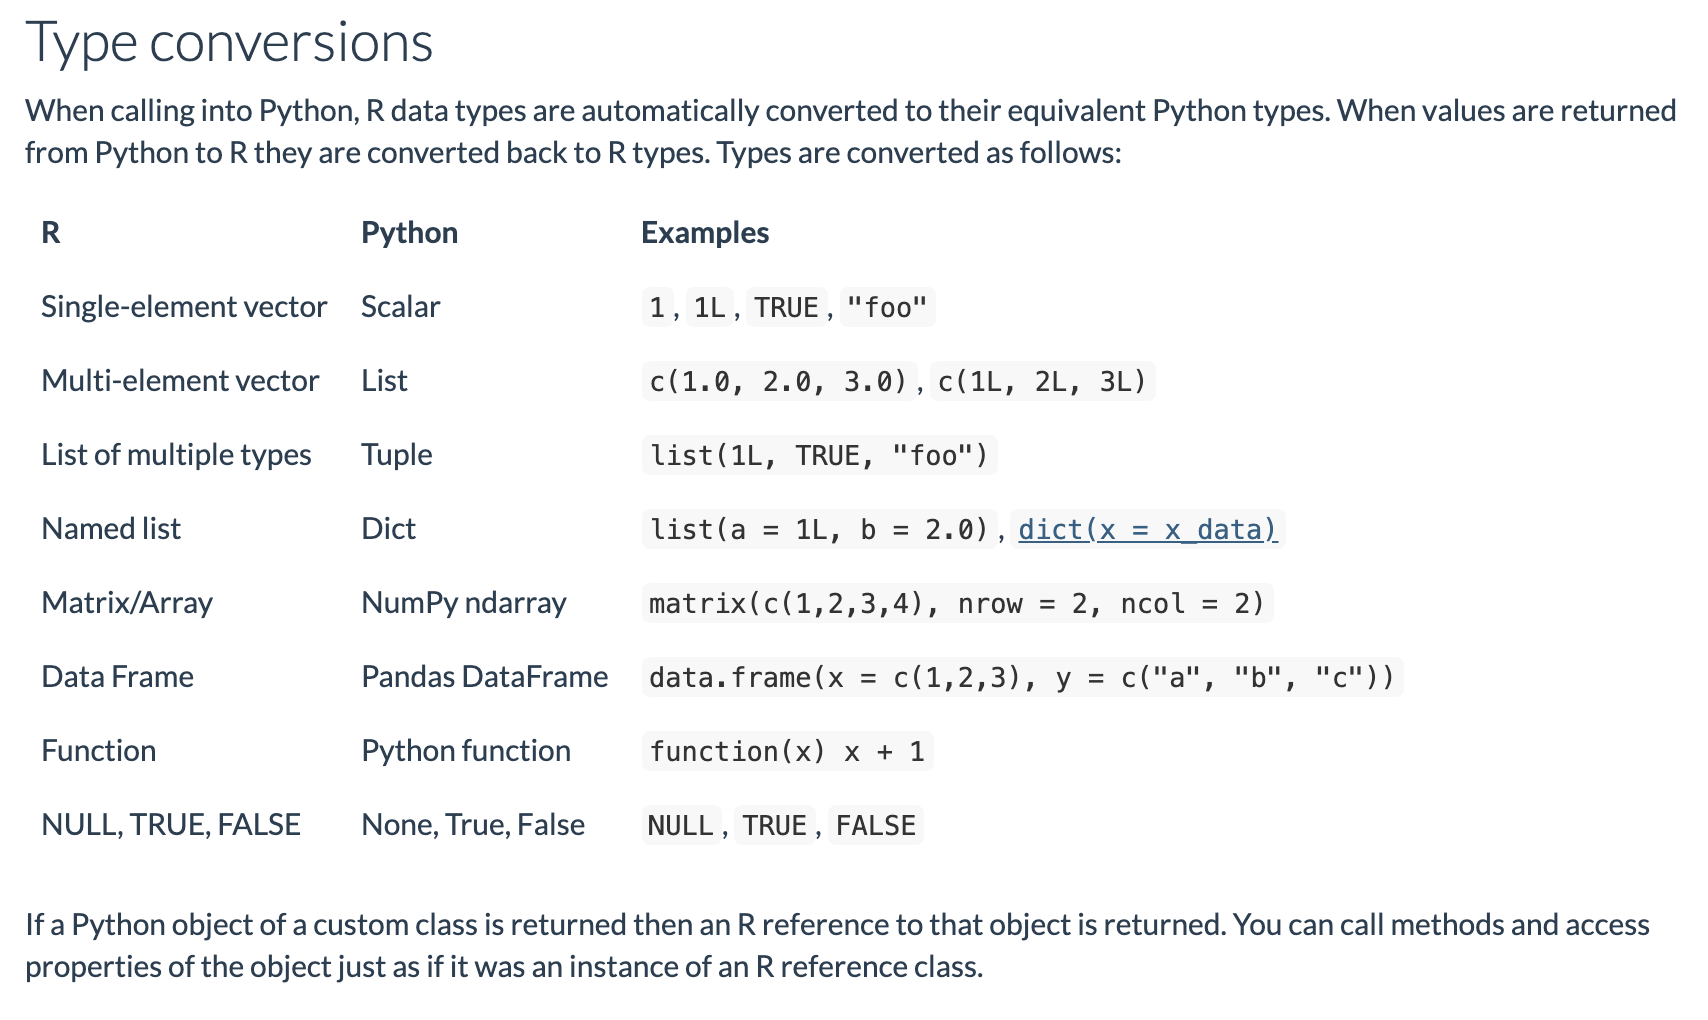
\includegraphics{_bookdown_files/reticulateconversions.png}

Client is the lowest level within the boto module, read more about it \href{https://boto3.amazonaws.com/v1/documentation/api/latest/reference/services/sns.html\#client}{here for sns}.

\begin{Shaded}
\begin{Highlighting}[]
\NormalTok{client <-}\StringTok{ }\NormalTok{boto}\OperatorTok{$}\KeywordTok{client}\NormalTok{(}\StringTok{'sns'}\NormalTok{, }\DataTypeTok{region_name=}\StringTok{'us-east-1'}\NormalTok{)}
\end{Highlighting}
\end{Shaded}

\begin{Shaded}
\begin{Highlighting}[]
\NormalTok{response <-}\StringTok{ }\NormalTok{client}\OperatorTok{$}\KeywordTok{publish}\NormalTok{(}
    \DataTypeTok{PhoneNumber=}\StringTok{"+15555555555"}\NormalTok{,}
    \DataTypeTok{Message=}\StringTok{"Hello World!!!!"}
\NormalTok{)}
\end{Highlighting}
\end{Shaded}

The AWS responses are pretty dirty. This is one of the issues I'm working on. We can take the response and clean it up for others.

\begin{Shaded}
\begin{Highlighting}[]
\NormalTok{response }
\end{Highlighting}
\end{Shaded}

\begin{verbatim}
## $ResponseMetadata
## $ResponseMetadata$RetryAttempts
## [1] 0
## 
## $ResponseMetadata$HTTPStatusCode
## [1] 200
## 
## $ResponseMetadata$RequestId
## [1] "2ab6b37b-21d9-5802-b257-e63d9900353f"
## 
## $ResponseMetadata$HTTPHeaders
## $ResponseMetadata$HTTPHeaders$`x-amzn-requestid`
## [1] "2ab6b37b-21d9-5802-b257-e63d9900353f"
## 
## $ResponseMetadata$HTTPHeaders$date
## [1] "Fri, 03 May 2019 21:46:01 GMT"
## 
## $ResponseMetadata$HTTPHeaders$`content-length`
## [1] "294"
## 
## $ResponseMetadata$HTTPHeaders$`content-type`
## [1] "text/xml"
## 
## 
## 
## $MessageId
## [1] "68561ace-e6fc-50e8-8b15-4f885e258dd5"
\end{verbatim}

While this is simplified, an R user will find this much more intuitive.

\begin{Shaded}
\begin{Highlighting}[]
\NormalTok{send_sms <-}\StringTok{ }\ControlFlowTok{function}\NormalTok{(}\DataTypeTok{phone_number =} \OtherTok{NA}\NormalTok{, }
                     \DataTypeTok{message =} \StringTok{"Hello World!"}\NormalTok{, }
                     \DataTypeTok{region =} \StringTok{"us-east-1"}\NormalTok{,}
                     \DataTypeTok{message_aws =} \OtherTok{FALSE}\NormalTok{) \{}
\NormalTok{  client <-}\StringTok{ }\NormalTok{boto}\OperatorTok{$}\KeywordTok{client}\NormalTok{(}\StringTok{'sns'}\NormalTok{, }\DataTypeTok{region_name=}\NormalTok{region)}
\NormalTok{  phone_number <-}\StringTok{ }\KeywordTok{paste0}\NormalTok{(}\StringTok{"+"}\NormalTok{, phone_number)}
\NormalTok{  response <-}\StringTok{ }\NormalTok{client}\OperatorTok{$}\KeywordTok{publish}\NormalTok{(}
      \DataTypeTok{PhoneNumber =}\NormalTok{ phone_number,}
      \DataTypeTok{Message     =}\NormalTok{ message}
\NormalTok{  )}
  \ControlFlowTok{if}\NormalTok{(message_aws) \{}
    \KeywordTok{return}\NormalTok{(response)}
\NormalTok{  \} }\ControlFlowTok{else}\NormalTok{ \{}
    \KeywordTok{return}\NormalTok{(}\OtherTok{TRUE}\NormalTok{)}
\NormalTok{  \}}
\NormalTok{\}}
\end{Highlighting}
\end{Shaded}

Doesn't this just seem a lot better? Wrapping up the most useful parts of Python code into R is the first step.

\begin{Shaded}
\begin{Highlighting}[]
\KeywordTok{send_sms}\NormalTok{(}\DataTypeTok{phone_number =} \DecValTok{15555555555}\NormalTok{, }\DataTypeTok{message =} \StringTok{"Hi, how are you?"}\NormalTok{)}
\end{Highlighting}
\end{Shaded}

\begin{verbatim}
## [1] TRUE
\end{verbatim}

\bibliography{book.bib,packages.bib}


\end{document}
